\begin{frame}{Régulation}
\framesubtitle{Interface avec les capteurs et actuateurs}
\begin{itemize}
  \item Moteurs:
  \begin{itemize}
  \item Commandés en PWM\\
  $\Rightarrow$ Signal de commande généré par le module output compare, à configurer
  \item Limitations physiques fixent le point de fonctionnement de la régulation
  \item Peu linéaires, dissymétriques
  \end{itemize}
\end{itemize}
\end{frame}

\begin{frame}{Régulation}
\framesubtitle{Interface avec les capteurs et actuateurs}
\begin{itemize}
  \item Encodeurs:
  \begin{itemize}
    \item $2\times90$ flancs montants par tour de roue\\
    $\Rightarrow$Signaux interprétés par le module QEI, à configurer
    \item Pas d'index hardware\\
    $\Rightarrow$ Index software pour rendre impossible l'overflow des compteurs
    \item Précision largement suffisante compte tenu de celle des moteurs
  \end{itemize}
\end{itemize}
\end{frame}

\begin{frame}{Régulation}
\framesubtitle{Mise en place de la boucle fermée}
\begin{itemize}
  \item Régulation numérique, $f_{regul} = \SI{100}{\hertz}$\\
  $\Rightarrow$ Timer. Actions de la routine:
  \begin{itemize}
    \item Lecture des encodeurs
    \item Calcul du rapport cyclique et commande des moteurs
    \item Mise à jour des consignes
    \item Détection de l'arrivée à la position visée
  \end{itemize}
\end{itemize}
\end{frame}

\begin{frame}{Régulation}
\framesubtitle{Choix du schéma de régulation}
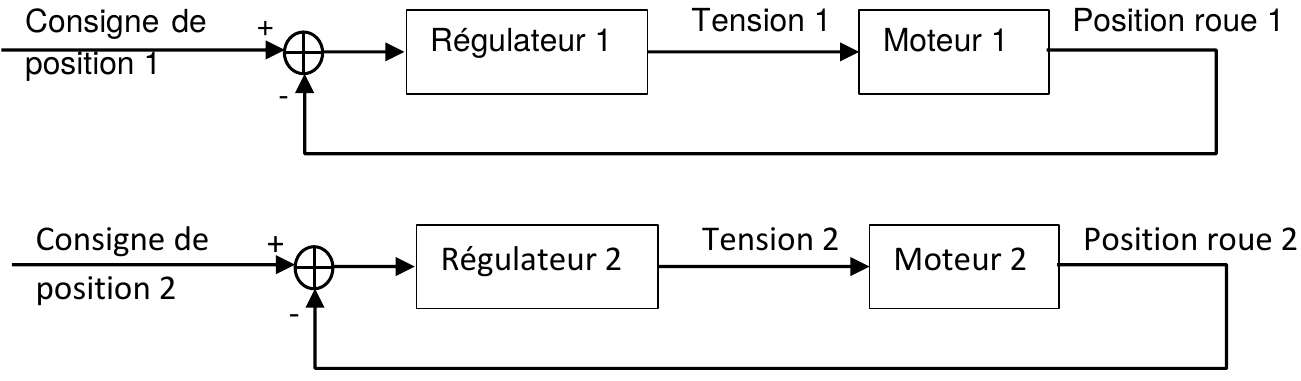
\includegraphics[width = \textwidth]{regulSISO.png}
\end{frame}

\begin{frame}{Régulation}
\framesubtitle{Choix du schéma de régulation}
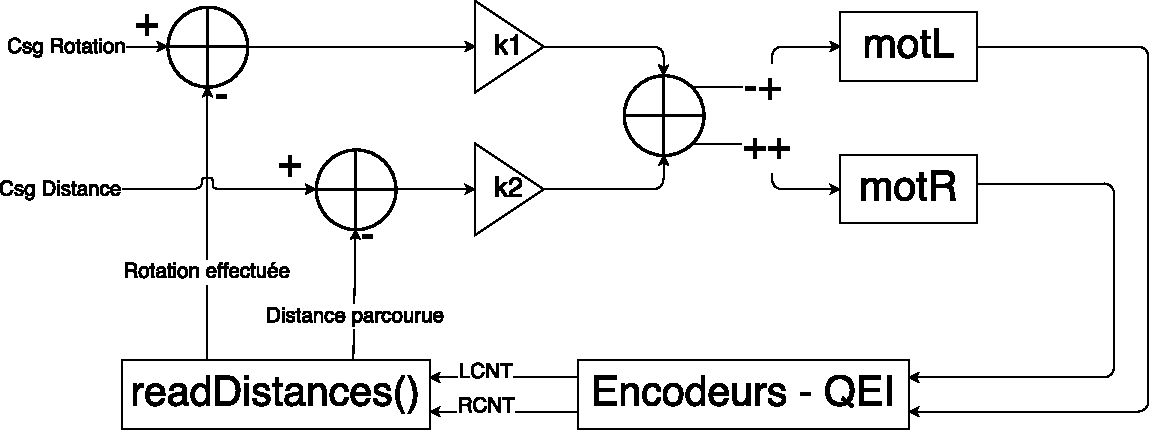
\includegraphics[width = \textwidth]{regulMIMO.pdf}
\end{frame}
